\chapter{Akwizycja i wykorzystanie danych z czujników ruchu}

Wprowadzone oznaczenia, w celu zwiększenia czytelności macierzy rotacji
$$
    \begin{array}{ccc}
        s_{\varphi} = sin\varphi, & s_{\theta} = sin\theta, & s_{\psi} = sin\psi \\
        c_{\varphi} = cos\varphi, & c_{\theta} = cos\theta, & c_{\psi} = cos\psi
    \end{array}
$$

Macierze rotacji
$$
    \mathbf{R_x(\varphi)} =
    \left[
        \begin{array}{ccc}
            1 & 0 & 0 \\
            0 & c_{\varphi} & s_{\varphi} \\
            0 & -s_{\varphi} & c_{\varphi}
        \end{array}
    \right]
    %
    \mathbf{R_y(\theta)} =
    \left[
        \begin{array}{ccc}
            c_{\theta} & 0 & -s_{\theta} \\
            0 & 1 & 0 \\
            s_{\theta} & 0 & c_{\theta}
        \end{array}
    \right]
    %
    \mathbf{R_z(\psi)} =
    \left[
        \begin{array}{ccc}
            c_{\psi} & s_{\psi} & 0 \\
            -s_{\psi} & c_{\psi} & 0 \\
            0 & 0 & 1
        \end{array}
    \right]
$$
%
$$
    \mathbf{R} =
    \mathbf{R_x(\varphi)R_y(\theta)R_z(\psi)} =
    \left[
        \begin{array}{ccc}
            c_{\theta}c_{\psi} & c_{\theta}s_{\psi} & s_{\theta} \\
            c_{\psi}s_{\theta}s_{\varphi} - s_{\varphi}s_{\psi} & c_{\varphi}c_{\psi} + s_{\theta}s_{\varphi}s_{\psi} & c_{\theta}s_{\varphi} \\
            c_{\varphi}c_{\psi}s_{\theta} + s_{\varphi}s_{\psi} & c_{\varphi}s_{\theta}s_{\psi} - c_{\psi}s_{\varphi} & c_{\theta}c_{\varphi}
        \end{array}
    \right]
$$
%----------------------------------------------------------------------------------------------------------------
\section{Żyroskop}

\begin{figure}[!htb]
    \centering
    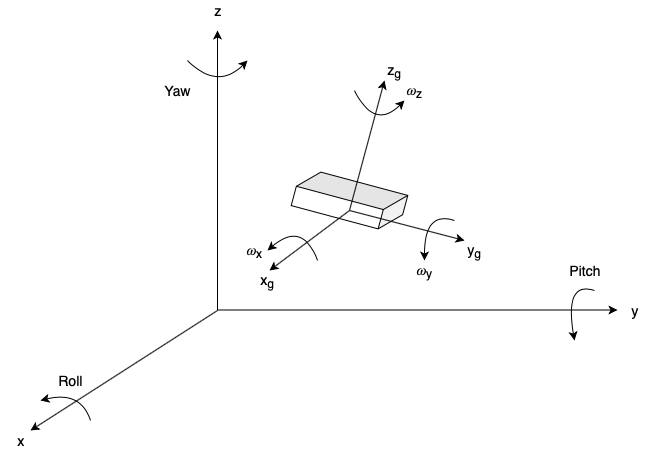
\includegraphics[width=0.6\textwidth]{Rysunki/Rozdzial03/Zyroskop.png}
    \caption{Wizualizacja odczytów żyroskopu}
\end{figure}

Wektor prędkości kątowych
$$
    \mathbf{\omega} = 
    \left[
    \begin{array}{c}
        \omega_x \\
        \omega_y \\
        \omega_z
    \end{array}
    \right]
$$

W przypadku, w którym interesuje nas jednowymiarowe określenie orientacji, możemy go wyznaczyć poprzez scałkowanie prędkości kątowej w danej osi \cite{Akwizycja}
$$
    \alpha_t = \int_{0}^{t} \omega \Delta t = \alpha_{t-1} + \omega_t \Delta t
$$

Problem pojawia się w momencie, w którym chcemy znać orientację czujnika w przestrzeni trójwymiarowej. Żyroskop mierzy prędkości kątowe w osiach swojego lokalnego układu współrzędnych i jeśli dokona się zmiany orientacji czujnika względem układu, w którym wyznaczamy orientację, to wyniki będą niepoprawne. W takim przypadku, należy skorzystać ze wzoru na prędkość kątową w przestrzeni, korzystając z własności $R^T=R^{-1}$, która wynika z tego, że macierz R jest ortogonalna.
\begin{equation}
    \left[\omega\right] = \dot{R}R^T \Rightarrow \dot{R} = R \left[\omega\right]
    \label{Predkosc obrotowa}
\end{equation}
gdzie
$$
    \mathbf{\left[\omega\right]} = 
    \left[
    \begin{array}{ccc}
        0 & -\omega_z & \omega_y \\
        \omega_z & 0 & -\omega_x \\
        -\omega_y & \omega_x & 0
    \end{array}
    \right]
$$
Elementami równania (\ref{Predkosc obrotowa}), które chcemy wyznaczyć są elementy macierzy \textbf{R}. Dokonuje się tego poprzez zapisanie równania w postaci równania różniczkowego
$$
\dot{R} = R\left[\omega\right]
$$
którego rozwiązaniem jest
$$
    R_t \approx R_{t-1}(I_{3x3}+\left[\omega\right] \Delta t)
$$

$$
    \left[
    \begin{array}{ccc}
        r_{11} & r_{12} & r_{13} \\
        r_{21} & r_{22} & r_{23} \\
        r_{31} & r_{32} & r_{33} \\
    \end{array}
    \right]_t
    =
    \left[
    \begin{array}{ccc}
        r_{11} & r_{12} & r_{13} \\
        r_{21} & r_{22} & r_{23} \\
        r_{31} & r_{32} & r_{33} \\
    \end{array}
    \right]_{t-1}
    %
    \left[
    \begin{array}{ccc}
        1 & -\omega_z\Delta t & \omega_y\Delta t \\
        \omega_z\Delta t & 1 & -\omega_x\Delta t \\
        -\omega_y\Delta t & \omega_x\Delta t & 1 \\
    \end{array}
    \right]
$$
gdzie macierz \textbf{R} w chwili $t=0$ dla zerowych wartości kątów, wynosi
$$
    \mathbf{R_{0}} =
    \left[
    \begin{array}{ccc}
        1 & 0 & 0 \\
        0 & 1 & 0 \\
        0 & 0 & 1
    \end{array}
    \right]
$$

Mając rozwiązanie równania różniczkowego, możemy obliczyć elementy macierzy $R_t$ oraz kąty Eulera na podstawie odpowiednich elementów tej macierzy
\begin{equation}
    \begin{array}{c}
        Roll(\varphi) = arctan(\frac{r_{32}}{r_{33}}) \\ \\
        Pitch(\theta) = arcsin(-r_{31}) \\ \\
        Yaw(\psi) = arctan(\frac{r_{21}}{r_{11}})
    \end{array}
\end{equation}

%----------------------------------------------------------------------------------------------------------------
\clearpage
\section{Akcelerometr}

\begin{figure}[!htb]
    \centering
    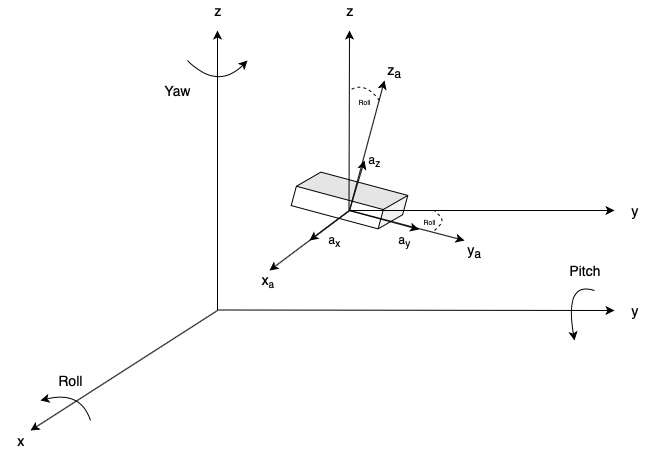
\includegraphics[width=0.6\textwidth]{Rysunki/Rozdzial03/Akcelerometr.png}
    \caption{Wizualizacja odczytów akcelerometru}
\end{figure}

Wektor przyspieszeń w osiach akcelerometru
$$
    \mathbf{a} = 
    \left[
    \begin{array}{cc}
        a_x \\
        a_y \\
        a_z
    \end{array}
    \right]
$$

Znormalizowany wektor równoległy do osi Z
$$
    \mathbf{(g_z)} =
    \left[
        \begin{array}{c}
            0 \\
            0 \\
            1
        \end{array}
    \right]
$$

Orientacja w przestrzeni RPY znormalizowanego wektora grawitacji
$$
R g_z = 
\left[
    \begin{array}{ccc}
        c_{\theta}c_{\psi} & c_{\theta}s_{\psi} & s_{\theta} \\
        c_{\psi}s_{\theta}s_{\varphi} - s_{\varphi}s_{\psi} & c_{\varphi}c_{\psi} + s_{\theta}s_{\varphi}s_{\psi} & c_{\theta}s_{\varphi} \\
        c_{\varphi}c_{\psi}s_{\theta} + s_{\varphi}s_{\psi} & c_{\varphi}s_{\theta}s_{\psi} - c_{\psi}s_{\varphi} & c_{\theta}c_{\varpi}
    \end{array}
\right]
\left[
    \begin{array}{c}
        0 \\
        0 \\
        1
    \end{array}
\right]
= 
\left[
    \begin{array}{c}
        -s_{\theta} \\
        c_{\theta}s_{\varphi} \\
        c_{\theta}c_{\varphi}
    \end{array}
\right]
$$

Orientację akcelerometru mierzy się względem wektora grawitacji, dzięki czemu można zapisać, że
\begin{equation}
    \mathbf{a} =
    \left[
        \begin{array}{c}
            -s_{\theta} \\
            c_{\theta}s_{\varphi} \\
            c_{\theta}c_{\varphi}
        \end{array}
    \right]
    \Rightarrow
    n
    \left[
        \begin{array}{c}
            a_x \\
            a_y \\
            a_z
        \end{array}
    \right]
    =
    \left[
        \begin{array}{c}
            -s_{\theta} \\
            c_{\theta}s_{\varphi} \\
            c_{\theta}c_{\varphi}
        \end{array}
    \right]
    \label{Orientacja akcelerometru}
\end{equation}
\\
gdzie
\begin{itemize}
    \item $a_x$ -- odczyt akcelerometru w osi x
    \item $a_y$ -- odczyt akcelerometru w osi y
    \item $a_z$ -- odczyt akcelerometru w osi z
    \item $n = \frac{1}{\sqrt{a_x^2 + a_y^2 + a_z^2}}$ 
\end{itemize}

Korzystając ze wzoru (\ref{Orientacja akcelerometru}) zapisujemy go w postaci układu równań
$$
    \left\{
        \begin{array}{l}
            na_x = -sin\theta\\
            na_y = cos\theta sin\varphi\\
            na_z = cos\theta cos\varphi
        \end{array}
    \right.
    \Rightarrow
    \left\{
        \begin{array}{l}
            sin\theta = -na_x \\
            cos\theta = n\sqrt{a_y^2 + a_z^2} \\
            sin\varphi = \frac{na_y}{cos\theta} \\
            cos\varphi = \frac{na_z}{cos\theta}
        \end{array}
    \right.
$$
i wyliczamy zależności trygonometryczne, z których otrzymujemy rotacje akcelerometru względem osi x oraz y
\begin{equation}
    \begin{array}{l}
        tg\varphi = \frac{sin\varphi}{cos\varphi} = \frac{a_y}{a_z} \Rightarrow Roll(\varphi) = arctg(\frac{a_y}{a_z}) \\ \\
        tg\theta = \frac{sin\theta}{cos\theta} = \frac{-a_x}{\sqrt{a_y^2+a_z^2}} \Rightarrow Pitch(\theta) = arctg\left(\frac{-a_x}{\sqrt{a_y^2+a_z^2}}\right)
    \end{array}
\end{equation}

Niestety, ale z racji tego, że orientację akcelerometru wyliczamy względem wektora grawitacji nie ma możliwości obliczenia rotacji względem osi Z, czyli kąta Yaw($\psi$).

%----------------------------------------------------------------------------------------------------------------
\section{Magnetometr}

\begin{figure}[h!]
    \centering
    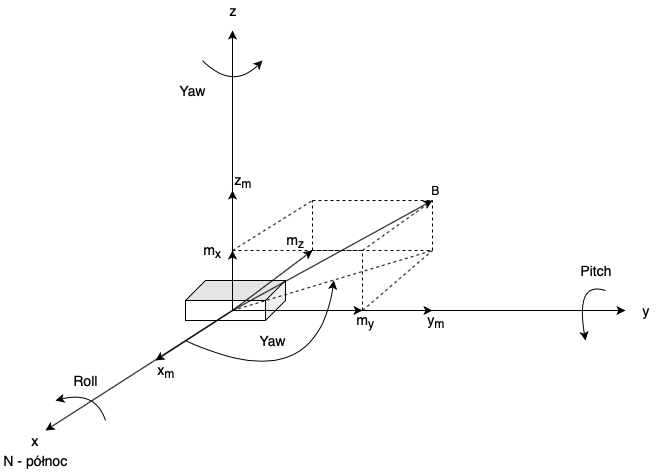
\includegraphics[width=0.6\textwidth]{Rysunki/Rozdzial03/Magnetometr.png}
    \caption{Wizualizacja odczytów magnetometru}
    \label{Rotacja magnetometru}
\end{figure}

\begin{figure}[h!]
    \centering
    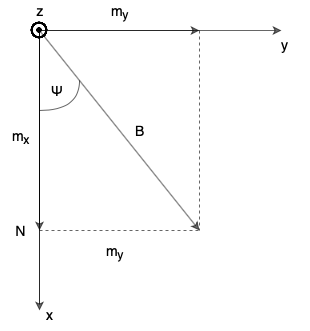
\includegraphics[width=0.3\textwidth]{Rysunki/Rozdzial03/Magnetometr_odchylenie.png}
    \caption{Odchylenie magnetometru od wektora północy magnetycznej}
    \label{Rotacja magnetometru}
\end{figure}

Wektor pola magnetycznego (odczyty magnetometru)
$$
    \mathbf{B} = 
    \left[
    \begin{array}{c}
        m_x \\
        m_y \\
        m_z
    \end{array}
    \right]
$$

Rotacja magnetometru wokół osi Z (odchylenie od wektora pola magnetycznego), przy założeniu, że wartości kątów Roll i Pitch są zerowe (brak odchylenia magnetometru od płaszczyzny XY)
\begin{equation}
    tg\psi = \frac{sin\psi}{cos\psi} = \frac{m_y}{m_x} \Rightarrow Yaw(\delta) = arctg\left(\frac{m_y}{m_x}\right)
    \label{Odchylenie magnetometru}
\end{equation}

Niestety w przypadku, w którym odchylimy magnetometr względem osi x lub y, obliczona według wzoru (\ref{Odchylenie magnetometru}) wartość obrotu wokół osi Z będzie nieprawidłowa, ponieważ zmieni się odczyt magnetometru w osiach x i y oraz z. W celu zniwelowania tego efektu dokonuje się kompensacji kąta wychylenia magnetometru.

%----------------------------------------------------------------------------------------------------------------
\subsection{Kompensacja kąta wychylenia}
Kompensacja kąta wychylenia magnetometru, to nic innego jak uwzględnienie w obliczeniach rotacji wokół osi x i y, wyznaczonych, np. za pomocą akcelerometru.

Wektor pola magnetycznego po kompensacji kąta wychylenia
\begin{equation}
    \begin{array}{c}
        \mathbf{B^{k}} = R_x(\varphi)R_y(\theta)B 
        \\ \\
        \left[
            \begin{array}{c}
                b^k_x \\
                b^k_y \\
                b^k_z
            \end{array}
        \right]
        =
        \left[
            \begin{array}{ccc}
                c_{\theta} & 0 & -s_{\theta} \\
                s_{\varphi}s_{\theta} & c_{\varphi} & s_{\varphi}c_{\theta} \\
                c_{\varphi}s_{\theta} & -s_{\varphi} & c_{\varphi}c_{\theta}
            \end{array}
        \right]
        \left[
            \begin{array}{c}
                m_x \\
                m_y \\
                m_z
            \end{array}
        \right]
        =
        \left[
            \begin{array}{c}
                c_{\theta}m_x - s_{\theta}m_z \\
                s_{\varphi}s_{\theta}m_x + c_{\varphi}m_y + s_{\varphi}c_{\theta}m_z \\
                c_{\varphi}s_{\theta}m_x - s_{\varphi}m_y + c_{\varphi}c_{\theta}m_z
            \end{array}
        \right]
    \end{array}
\end{equation}

Rotacja magnetometru wokół osi Z (odchylenie od wektora pola magnetycznego), po kompensacji kąta wychylenia magnetometru
\begin{equation}
    Yaw(\psi) = arctg\left(\frac{b^k_y}{b^k_x}\right) = arctg\left(\frac{s_{\varphi}s_{\theta}m_x + c_{\varphi}m_y + s_{\varphi}c_{\theta}m_z}{c_{\theta}m_x - s_{\theta}m_z}\right)
    \label{Odchylenie po kompensacji}
\end{equation}

%----------------------------------------------------------------------------------------------------------------
\subsection{Deklinacja magnetyczna}
W celu uzyskania dokładniejszego pomiaru uzależnionego od aktualnej pozycji na Ziemi uwzględnia się deklinację magnetyczną, która dla Wrocławia wynosi
$$
    \delta = 4^{o}E8'E \approx 4,13^{o}E
$$
co daje ostateczną postać wzoru na wskazanie magnetometru, przy założeniu, że kąt Yaw obliczony jest w stopniach, a nie w radianach
$$
   Yaw(\psi) = Yaw(\psi) + \delta = Yaw(\psi) + 4,13^o 
$$

%----------------------------------------------------------------------------------------------------------------
\subsection{Kompensacja efektu ,,Hard Iron'' oraz ,,Soft Iron''}

Nieskalibrowane odczyty magnetometru zostały przedstawione na rysunku \ref{Magnetometr nieskalibrowany}. Na wykresach widoczne są elipsy przesunięte względem punktu (0,0) na wykresie. Odczyty dla skalibrowanego magnetometru na płaszczyznach XY, XZ oraz YZ powinny mieć swój środek w punkcie (0,0), czyli kulą o środku w punkcie (0,0,0) w przestrzeni XYZ.

\begin{figure}[h!]
    \centering
    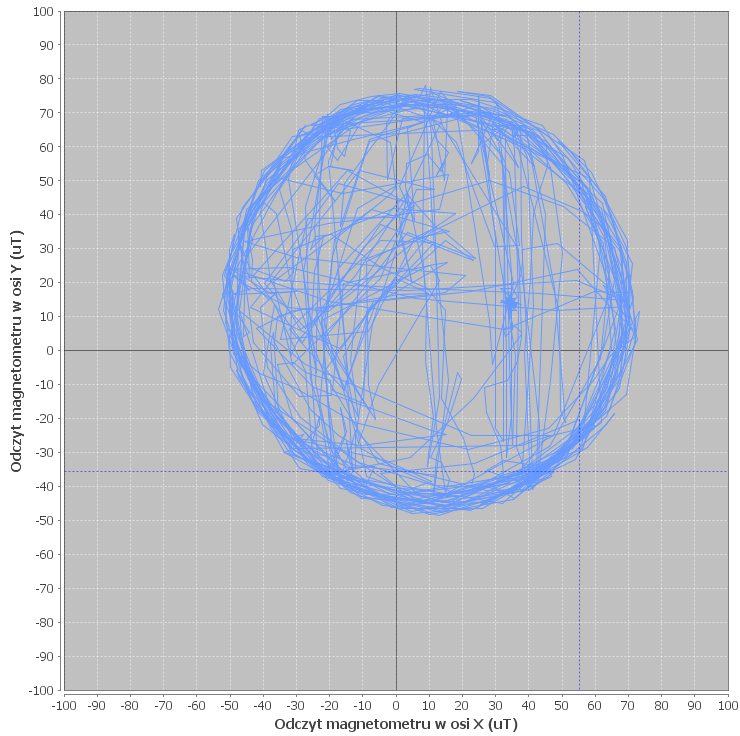
\includegraphics[width=0.5\textwidth]{Rysunki/Rozdzial03/Magnetometr_nieskalibrowany_XY.png}
    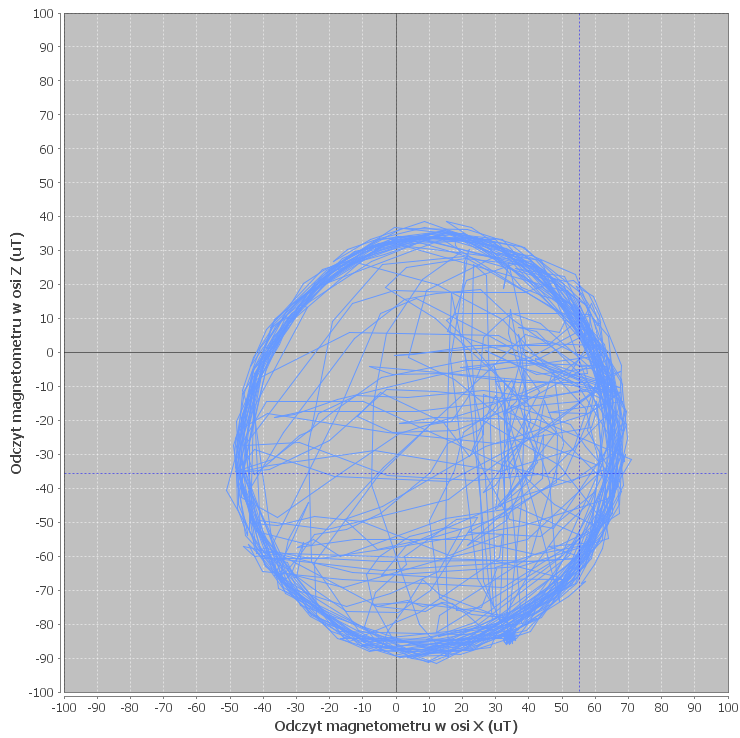
\includegraphics[width=0.5\textwidth]{Rysunki/Rozdzial03/Magnetometr_nieskalibrowany_XZ.png}
    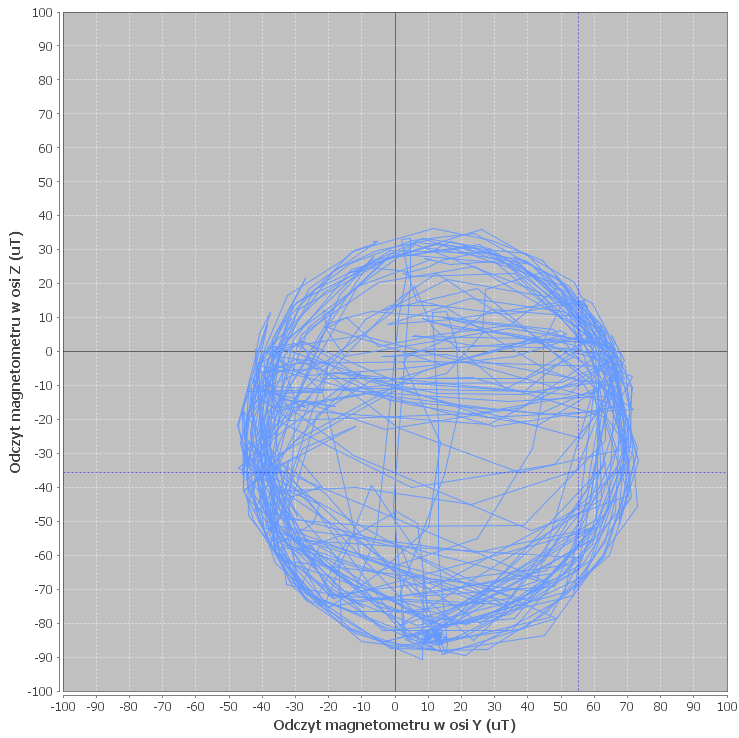
\includegraphics[width=0.5\textwidth]{Rysunki/Rozdzial03/Magnetometr_nieskalibrowany_YZ.png}
    \caption{Odczyty dla nieskalibrowanego magnetometru}
    \label{Magnetometr nieskalibrowany}
\end{figure}

Efekt ,,Hard Iron'' (wpływ ferromagnetyków twardych) kompensuje się poprzez przesunięcie odczytów na środek układu współrzędnych o wyznaczony offset. Przesunięcie wyznacza się na podstawie maksymalnej oraz minimalnej wartości odczytu w danej osi, według następujących wzorów
$$
    \begin{array}{c}
        offset(m_x) = \frac{max(m_x) + min(m_x)}{2} \\ \\
        offset(m_y) = \frac{max(m_y) + min(m_y)}{2} \\ \\
        offset(m_z) = \frac{max(m_z) + min(m_z)}{2}
    \end{array}
$$

Efekt ,,Soft Iron'' (wpływ ferromagnetyków miękkich), który objawia się zniekształceniem odczytów, które powinny tworzyć idealny okrąg na płaszczyźnie, należy skompensować przeskalowując odczyty o wartości wyliczane według następujących wzorów
$$
    \begin{array}{c}
        a(m_x) = \frac{max(m_x) - min(m_x)}{2}, a(m_y) = \frac{max(m_y) - min(m_y)}{2}, a(m_z) = \frac{max(m_z) - min(m_z)}{2} \\ \\
        b = \frac{a(m_x) + a(m_y) + a(m_z)}{3} \\ \\
        scale(m_x) = \frac{b}{a(m_x)}, scale(m_y) = \frac{b}{a(m_y)}, scale(m_z) = \frac{b}{a(m_z)} 
    \end{array}
$$

Na rysunku \ref{Magnetometr skalibrowany} widać, że odczyty dla magnetometru zostały skalibrowane. Przesunięcia odczytów we wszystkich osiach oraz delikatne zniekształcenie dla odczytu XZ zostały skompensowane. Ostateczną postać wektora odczytów magnetometru oblicza się według wzoru (\ref{Ostateczny wektor magnetometr})
\begin{equation}
    \begin{array}{c}
        \left[
            \begin{array}{c}
                m_x \\
                m_y \\
                m_z
            \end{array}
        \right]
        =
        \left[
            \begin{array}{c}
                m_x - offset(m_x) \\
                m_y - offset(m_y) \\
                m_z - offset(m_z)
            \end{array}
        \right]
        \left[
            \begin{array}{c}
                scale(m_x) \\
                scale(m_y) \\
                scale(m_z)
            \end{array}
        \right]
    \end{array}
    \label{Ostateczny wektor magnetometr}
\end{equation}

\begin{figure}[h!]
    \centering
    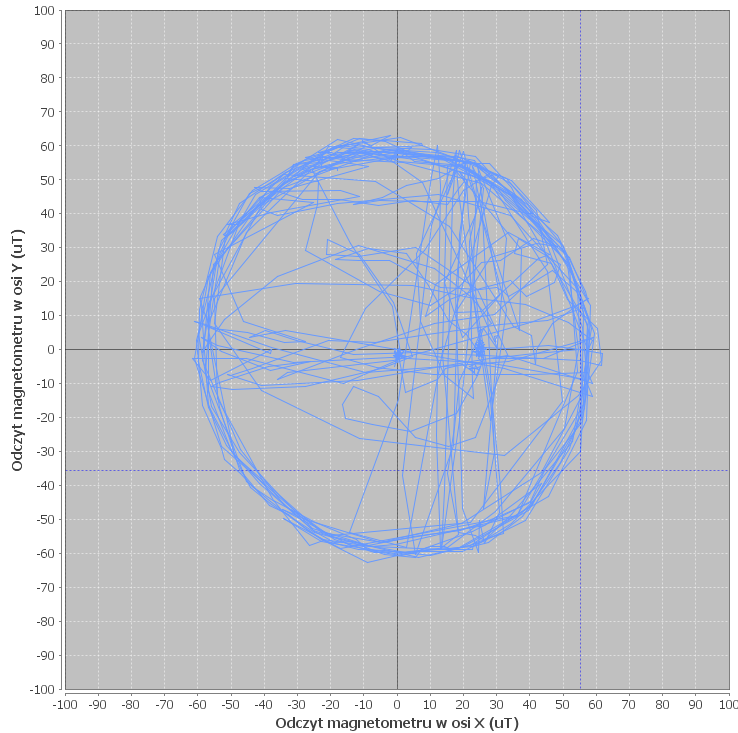
\includegraphics[width=0.5\textwidth]{Rysunki/Rozdzial03/Magnetometr_skalibrowany_hardiron_XY.png}
    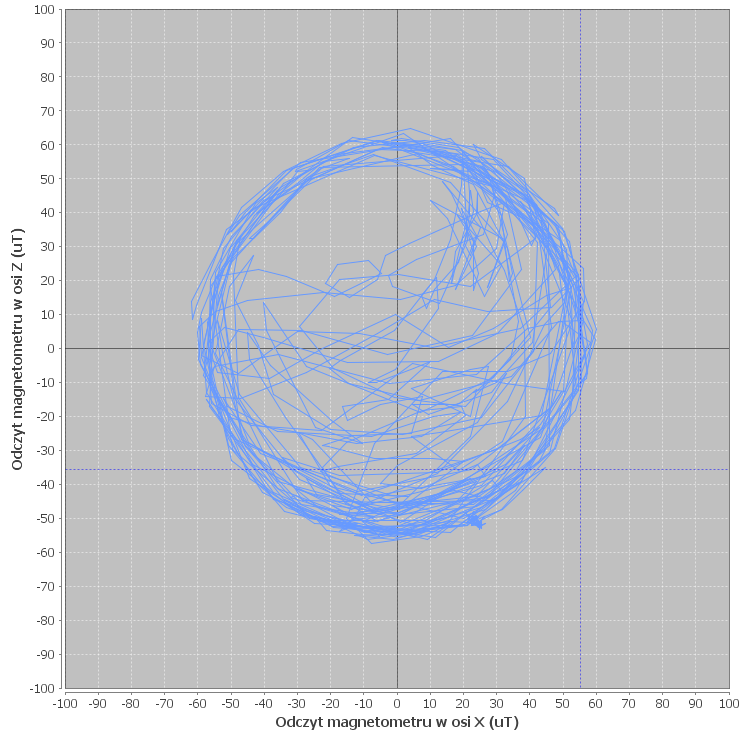
\includegraphics[width=0.5\textwidth]{Rysunki/Rozdzial03/Magnetometr_skalibrowany_hardiron_XZ.png}
    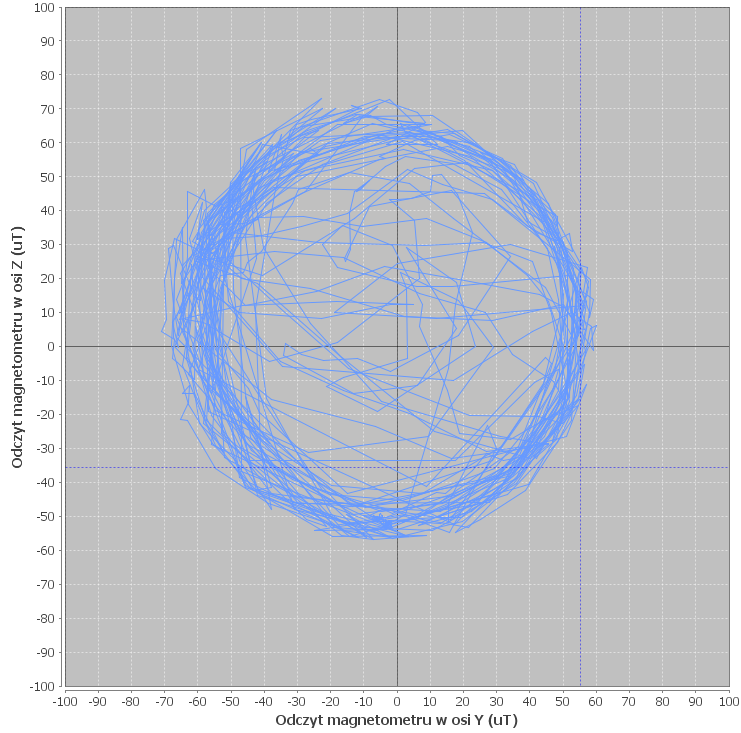
\includegraphics[width=0.5\textwidth]{Rysunki/Rozdzial03/Magnetometr_skalibrowany_hardiron_YZ.png}
    \caption{Odczyty dla skalibrowanego magnetometru}
    \label{Magnetometr skalibrowany}
\end{figure}

%----------------------------------------------------------------------------------------------------------------